% Fig. 2.16 / spec Fig A16 -- the three quartiles cut the distribution into
%   four parts of equal area (the q = 4 case of the k-th q-quantile).
% Source: mathstatch2.tex lines 2486-2526.  The manuscript picture there is,
%   geometrically, an exact copy of the one at lines 2438-2478 (Fig. 2.15):
%   same curve, same single boundary at 1.3, same single shaded block, only
%   the labels differ.  Ruling 7-C of CH2_SEC22_REWRITE.md keeps both figure
%   numbers and redraws this second one as a genuine four-way split, so that
%   the sentence "the q-1 quantiles cut the distribution into q equal parts"
%   finally has a picture.
%
% Numbers (Gamma(shape 4, rate 1.7), the chapter's right-skewed reference
% density of spec 1.6; f(x) = 1.3920167 x^3 e^{-1.7x}):
%   q_1 = 1.491365   f = 0.365865
%   q_2 = 2.160036   f = 0.356674   (the median, spec 1.6 gives 2.160035)
%   q_3 = 3.005546   f = 0.228254
%   peak at 3/1.7 = 1.764706, f = 0.380871
%   areas: F(q_1) = F(q_2) - F(q_1) = F(q_3) - F(q_2) = 0.250000 exactly;
%   the fourth block as drawn, [q_3, 6.4], is 0.244620, the missing 0.005380
%   being the tail beyond the plotted range.
%
% Deviations from CH2_FIGURE_SPECS.md:
%
% 1. Spec Fig A16 records the geometry of the manuscript picture and offers
%    two ways out of the duplication.  This file takes the second one (a real
%    four-way split) per ruling 7-C, so none of the coordinates of spec A16
%    are used.  Fig. 2.15 keeps the manuscript geometry and is a separate
%    file.
%
% 2. Spec 3.2 item 3 states that the 0.25 quantile of Gamma(4,1.7) is 1.578.
%    That value is wrong: F(1.578) = 0.282075, checked both by the closed form
%    for integer shape and by Simpson quadrature.  The true value is 1.491365.
%    Since Fig. 2.15 is meant to use the same p = 0.25 boundary, it has to use
%    1.491365 as well if the two figures are to agree.
%
% 3. Spec 1.2 caps fill opacity at 0.12 to 0.18.  The four blocks alternate
%    0.18 / 0.08, borrowing the 0.08 that spec 1.2 already lists for the
%    innermost step of nested shading.  Within 0.12-0.18 the alternation is
%    too faint to separate the blocks, and separating them by hue is ruled out
%    by spec 1.7.  The dashed boundaries carry the split as well, so the
%    shading is the second cue, not the only one.
%
% 4. The four blocks each carry a 1/4 label, which the manuscript's two
%    quantile pictures do not have (they label p and 1-p on either side of a
%    single boundary).  Without them the equality of the four areas has to be
%    taken on trust from the caption.
%
% 5. \DeclareMathSizes{10}{10}{9}{8} raises the math script sizes from the
%    default 7pt/5pt.  The smallest marks in the picture are the subscripts of
%    q_1, q_2, q_3 and the X of f_X; at 7pt they would show at 10.7px on a
%    390px phone, under the 12px floor of spec 1.3.  Native size is
%    206.796 x 110.284 pt (drawing range 7.15cm wide, inside the 9.0cm cap),
%    the bounding box being shared with median-intuition.tex and
%    quantile-intuition.tex so that the three figures drawn on this curve
%    render at one scale.  A mark of S pt shows at
%    S x 0.99626 x <display width> / 206.796 px:
%        display width      350px    309px    288.6px
%        10pt text          16.86    14.88    13.90
%        9pt scripts        15.18    13.40    12.51
%        8pt scriptscripts  13.49    11.91    11.12
%    The 350px column is the plain topic-figure--wide case, which is where
%    this figure lands if it sits in body text as it does in the manuscript;
%    the two narrower columns are the widths measured for figures inside an
%    example box and inside a doubly nested proof box.  The only mark at
%    scriptscript size is the X of f_X, a component of the symbol rather than
%    a label of its own, and it is already far above the 5pt the default
%    setting would have given it.
%
% 6. The boundaries are labelled q_1, q_2, q_3, following the manuscript's own
%    notation q_k for the k-th q-quantile (here q = 4).  Ruling 7-C writes
%    them as Q_1, Q_2, Q_3.  Changing them is a one-line edit if the author
%    prefers the capital.
\documentclass[tikz,border=2pt]{standalone}
\usepackage{amsmath}
\usepackage{amssymb}
\usepackage{xcolor}
\usetikzlibrary{arrows.meta}
\newcommand{\sssig}{\scriptscriptstyle}
\DeclareMathSizes{10}{10}{9}{8}

\definecolor{journalink}{HTML}{1F1C18}
\definecolor{journalmuted}{HTML}{8A7F72}
\definecolor{journalaccent}{HTML}{9C2D2D}

\begin{document}
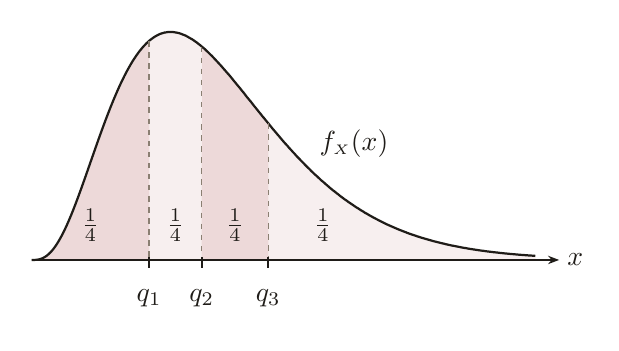
\begin{tikzpicture}[
  x=1cm,
  y=7.6cm,
  every node/.style={font=\normalsize, journalink},
  axis/.style={journalink, line width=0.8pt, -{Stealth[length=4pt]}},
  tick/.style={journalink, line width=0.8pt},
  curve/.style={journalink, line width=0.8pt},
  guide/.style={journalmuted, line width=0.5pt, dash pattern=on 2pt off 2pt},
  blockdark/.style={journalaccent, fill opacity=0.18},
  blocklight/.style={journalaccent, fill opacity=0.08}
]
  % ---- bounding box shared with median-intuition.tex and
  %      quantile-intuition.tex, which draw the same curve at the same scale
  \path (-0.05cm,-0.80cm) rectangle (7.10cm,2.95cm);

  % ---- the four blocks, each of area 1/4 -------------------------------
  % Shading paths follow spec 1.6: from the foot of the left boundary along
  % the x axis to the foot of the right boundary, up to the curve, back along
  % the curve, cycle.
  \fill[blockdark]
    (0,0) -- (1.491365,0) -- (1.491365,0.365865)
    -- plot[domain=1.491365:0, samples=200, smooth]
       (\x,{1.3920167*pow(\x*exp(-0.56666667*\x),3)}) -- cycle;
  \fill[blocklight]
    (1.491365,0) -- (2.160036,0) -- (2.160036,0.356674)
    -- plot[domain=2.160036:1.491365, samples=200, smooth]
       (\x,{1.3920167*pow(\x*exp(-0.56666667*\x),3)}) -- cycle;
  \fill[blockdark]
    (2.160036,0) -- (3.005546,0) -- (3.005546,0.228254)
    -- plot[domain=3.005546:2.160036, samples=200, smooth]
       (\x,{1.3920167*pow(\x*exp(-0.56666667*\x),3)}) -- cycle;
  \fill[blocklight]
    (3.005546,0) -- (6.4,0) -- (6.4,0.006872)
    -- plot[domain=6.4:3.005546, samples=200, smooth]
       (\x,{1.3920167*pow(\x*exp(-0.56666667*\x),3)}) -- cycle;

  % ---- density curve: Gamma(4, 1.7) ------------------------------------
  \draw[curve] plot[domain=0:6.4, samples=300, smooth]
    (\x,{1.3920167*pow(\x*exp(-0.56666667*\x),3)});

  % ---- x axis ----------------------------------------------------------
  \draw[axis] (0,0) -- (6.7,0);
  \node[anchor=west, inner sep=2.8pt] at (6.7,0) {$x$};

  % ---- the three quartiles ---------------------------------------------
  \draw[guide] (1.491365,0.365865) -- (1.491365,0);
  \draw[guide] (2.160036,0.356674) -- (2.160036,0);
  \draw[guide] (3.005546,0.228254) -- (3.005546,0);
  \foreach \q in {1.491365, 2.160036, 3.005546}
    \draw[tick] ([yshift=0.035cm]\q,0) -- ([yshift=-0.106cm]\q,0);
  \node[anchor=north] at ([yshift=-0.25cm]1.491365,0) {$q_{1}$};
  \node[anchor=north] at ([yshift=-0.25cm]2.160036,0) {$q_{2}$};
  \node[anchor=north] at ([yshift=-0.25cm]3.005546,0) {$q_{3}$};

  % ---- one quarter of the area in each block ---------------------------
  \node[inner sep=0pt] at ([yshift=0.44cm]0.746,0)  {$\frac{1}{4}$};
  \node[inner sep=0pt] at ([yshift=0.44cm]1.826,0)  {$\frac{1}{4}$};
  \node[inner sep=0pt] at ([yshift=0.44cm]2.583,0)  {$\frac{1}{4}$};
  \node[inner sep=0pt] at ([yshift=0.44cm]3.700,0)  {$\frac{1}{4}$};

  % ---- curve label -----------------------------------------------------
  \node[anchor=south west, inner sep=0pt] at ([yshift=1.30cm]3.65,0)
    {$f_{\sssig X}(x)$};
\end{tikzpicture}
\end{document}
